%----------------------------------------------------------------------------------------
%    PACKAGES AND THEMES
%----------------------------------------------------------------------------------------

\documentclass[aspectratio=169,xcolor=dvipsnames]{beamer}
\usetheme{SimpleDarkBlue}

\usepackage{hyperref} % Ajout de hyperref (corrigé)
\usepackage{graphicx} % Allows including images
\usepackage{booktabs} % Allows the use of \toprule, \midrule and \bottomrule in tables
\usepackage{natbib} % For citation commands like \citetitle

%----------------------------------------------------------------------------------------
%    TITLE PAGE
%----------------------------------------------------------------------------------------

\title{Notes}
\subtitle{}

\author{Julien Armand}

\institute
{
    Université Laval % Your institution for the title page
}
\date{\today} % Date, can be changed to a custom date

%----------------------------------------------------------------------------------------
%    PRESENTATION SLIDES
%----------------------------------------------------------------------------------------

\begin{document}

\AtBeginSection[]{
    \ifnum\value{section}=1
        \setbeamercolor{frametitle}{bg=MidnightBlue, fg=white}
    \fi
    \ifnum\value{section}=2
        \setbeamercolor{frametitle}{bg=ForestGreen, fg=white}
    \fi
    \ifnum\value{section}=3
        \setbeamercolor{frametitle}{bg=BrickRed, fg=white}
    \fi
    \ifnum\value{section}=4
        \setbeamercolor{frametitle}{bg=Goldenrod, fg=black}
    \fi
    \ifnum\value{section}=5
        \setbeamercolor{frametitle}{bg=RoyalBlue, fg=white}
    \fi
    \ifnum\value{section}=6
        \setbeamercolor{frametitle}{bg=Orchid, fg=black}
    \fi
    \ifnum\value{section}=7
        \setbeamercolor{frametitle}{bg=Teal, fg=white}
    \fi
}

\begin{frame}
    % Print the title page as the first slide
    \titlepage
\end{frame}

\begin{frame}{Overview}
    % Throughout your presentation, if you choose to use \section{} and \subsection{} commands, 
    % these will automatically be printed on this slide as an overview of your presentation
    \tableofcontents
\end{frame}

%------------------------------------------------
\section{Éléments clés}
%------------------------------------------------
\begin{frame}{Tests}

\end{frame}


\begin{frame}{Bullet Points}
    \begin{itemize}
        \item Feedback loop 
        \item MARL
        \item Théorie des jeux
    \end{itemize}
\end{frame}

\begin{frame}{Classification des feedbacks loops}
    \begin{itemize}
        \item sampling (assistant vocaux (native/non-native))
        \item individual (algo force les gens a changer pour s'adapter)
        \item label (mentir pour influencer un algoritme)
        \item model (apple tasting/bank loan problem/hiring algo/)
        \item outcome (la prédiction influence le résultat le médecin qui donne des soins de fin de vie à ceux qui ont de grandes chances de mourir/ the loan might be granted, but at a higher interest rate)
        \item adversarial or not 
        \item 
positive feedback loop (also known as reinforcing)  negative feedback loop
(also known as balancing) a
\item Representation bias ( Sampling, ML model)
\item Individual (Historical bias)
\item Measurement bias (Feature, Outcome)
    \end{itemize}
        (\href{http://dx.doi.org/10.1145/3617694.3623227}{\color{blue} Classification des feedbacks loops})
\end{frame}
%------------------------------------------------

%------------------------------------------------
\section{Lectures sur la théorie des jeux}
%------------------------------------------------

\begin{frame}{Théorie des jeux}
    \begin{itemize}
        \item zero sum game
        \item Équilibre de Nash (fort/faible)
        \item Équilibre minmax
        \item  \href{https://fr.wikipedia.org/wiki/Strat\%C3\%A9gie_\%C3\%A9volutivement_stable}{\color{blue} stratégie évolutivement stable}
        \item Jeu de Markov
        \item Disk game
        \item monotonic
        
    \end{itemize}
\end{frame}


\begin{frame}{Liste rapides de jeu}
    \begin{itemize}
        \item game of chiken
        \item hawk-dove
        \item (iterated) prisonner dilema
        \item Pour certains paramètres, un jeu de chiken peut devenir un jeu de hawk-dove, ou un jeu de hawk-dove un jeu du dileme du prisonnier
    \end{itemize}
\end{frame}

\begin{frame}{Roche papier ciseaux}

    \begin{itemize}
        \item Dynamique dans le monde animal: lézard(ajout source) (un autre aussi voir les trois du paper sur la spatialité avec des population de E.coli) \href{https://www.nature.com/articles/306368a0}{\color{blue} S. cerevisiae.}
        \item roche papier ciseaux possède un Evolutionarily Unstable Nash Equilibrium / Heteroclinic Cycle
    \end{itemize}

\end{frame}

\begin{frame}{Théorie}

    \begin{itemize}
        \item les EGT (evolutionnary game)  s'analysent avec \href{ https://en.wikipedia.org/wiki/Replicator_equation}{\color{blue} replicator equation}
        \href{https://www.researchgate.net/publication/221454784_A_selection-mutation_model_for_q-learning_in_multi-agent_systems}{ \color{blue} Analyse théorique avec Q learning an the replicator system}
        
        \item MAB bernoulli non-stationnary environnemnt (fixe une limite sur la quantité de changements possibles sur les probabilités des bras et analyse les bornes sur le regret) 
\href{https://proceedings.neurips.cc/paper_files/paper/2014/file/903ce9225fca3e988c2af215d4e544d3-Paper.pdf}{\color{blue} Stochastic Multi-Armed-Bandit Problem
with Non-stationary Rewards}
        \end{itemize}
\end{frame}
\begin{frame}{Théorie}
    \begin{itemize}
        \item Sur les cycles en théorie des jeux : 
        \href{https://arxiv.org/pdf/2305.13619}{\color{blue} Heteroclinic Orbits to Nash Equilibrium} AAAI 2024.
        \item Dans les systèmes dynamiques, le framework utilisé pour l'analyse des feedback loops : 
        \href{https://en.wikipedia.org/wiki/Heteroclinic_cycle}{\color{blue} Heteroclinic cycle}.
        \item \href{https://arxiv.org/abs/2410.17466}{\color{blue} Evolution with Opponent-Learning Awareness} : Multi-agent policy gradient (replicator dynamic), hawk dove, roche papier ciseaux.
        \item \href{https://arxiv.org/abs/1901.08106}{\color{blue} Cyclic game/setting/preuve générale pour des agents avec un réseau de neurones}.
        \item \href{https://www.fields.utoronto.ca/talks/Stochastic-Variant-Replicator-Dynamics-Zero-Sum-Games-and-Its-Invariant-Measures}{\color{blue} A Stochastic Variant of Replicator Dynamics in Zero-Sum Games and Its Invariant Measures} : Matching Pennies/Analyse poussée.
        \item "The Nash Equilibrium of an RPS game is relatively simple but computationally intractable; hence, various algorithms are employed to converge to a state of maximum payoff. In this paper, five algorithms, namely - Counterfactual Regret Minimization, Monte Carlo Tree Search, Q-learning, Deep Q-Network and Proximal Policy Optimization" : 
        \href{https://www.researchgate.net/publication/378246505_Convergence_to_Nash_Equilibrium_A_Comparative_Study_of_Rock-Paper-Scissors_Algorithms}{\color{blue} Convergence to Nash Equilibrium: A Comparative Study of Rock-Paper-Scissors Algorithms}. exp3 auteur année titre conférence
    \end{itemize}
\end{frame}

\begin{frame}{Théorie}
    \begin{itemize}
        \item \href{https://www.pnas.org/doi/epdf/10.1073/pnas.032086299}{\color{blue} Chaos in learning a simple two-person game} Hamiltonian chaos RPS 2002
    \end{itemize}
\end{frame}

\begin{frame}{vidéos intéressantes}

    \begin{itemize}
    \item \href{https://www.youtube.com/watch?v=tCoEYFbDVoI}{\color{blue} simulation évolution de roche papier ciseau} 
    \item \href{https://www.youtube.com/watch?v=YKB763gy3pc}{\color{blue} vidéo explicative sur une stratégie évolutivement instable pour le jeu Hawk-Dove}
    \item \href{https://youtu.be/vAOuy21n4tc?si=DvrjIaCqho_XKwWs&t=110}{\color{blue} Rock-Paper-Scissors equation on the sphere} \href{https://www.nature.com/articles/nature00823}{\color{blue} Rock-Paper-Scissors equation on the sphere}
    \end{itemize}

\end{frame}

\begin{frame}{autres concepts}
\begin{itemize}
    \item Lyapunov functions
    \item Lokta-Volteri
    \item processus stochastique
\end{itemize}
\end{frame}

%------------------------------------------------
\section{Autres}
%------------------------------------------------

\begin{frame}{article pt à lire}
    \href{https://proceedings.neurips.cc/paper/2016/file/962e56a8a0b0420d87272a682bfd1e53-Paper.pdf}{\color{blue} Deconvolving Feedback Loops
in Recommender Systems
}
\end{frame}

\begin{frame}{Nouvel ajout à ce document}
\begin{itemize}
    \item 17 mars 2018
    \item Meilleurs figures tirés de revues de la littérature
\end{itemize}
\end{frame}

\begin{frame}{Listes des reviews à discuter}
\begin{itemize}
    \item Repeteated Game (2011) : \citet{crandall_learning_2011}
    \item Evolutionnary game (2015):
    \citet{bloembergen_evolutionary_2015}
    \item Multi-agent general \cite{hernandez-leal_survey_2019}
    \item Markov game (2012): \citet{matignon_independent_2012}
\end{itemize}
\end{frame}

\begin{frame}{Repeated game}

  \begin{figure}
    \centering
    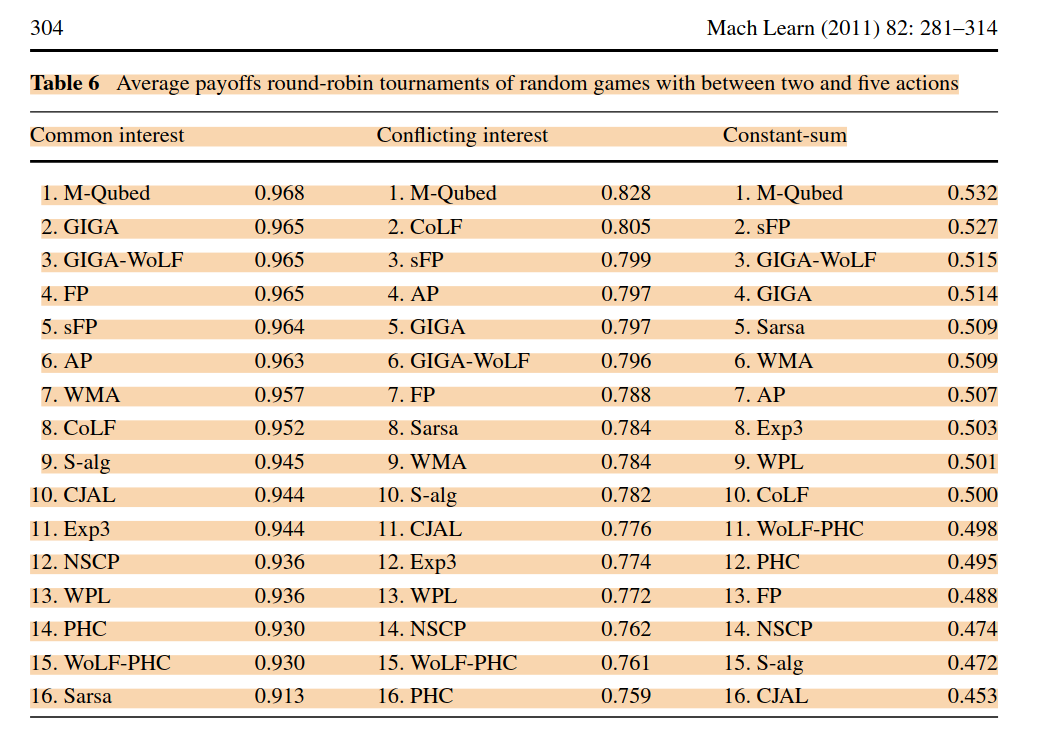
\includegraphics[scale=0.20]{round-robin tournaments.png}
    \caption{\citet{crandall_learning_2011} Learning to compete, coordinate, and
cooperate in repeated games using reinforcement learning}
  \end{figure}
\end{frame}

\begin{frame}{Evolutionnary game theory}
  \begin{figure}
    \centering
    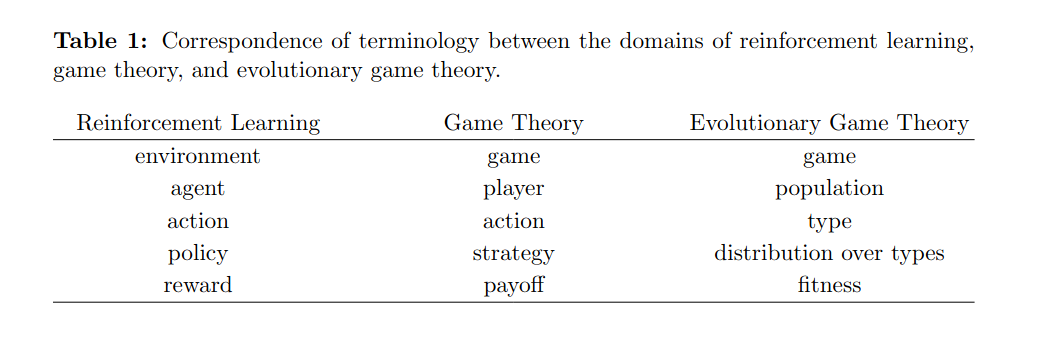
\includegraphics[scale=0.30]{Terminology.png}
    \caption{\citet{bloembergen_evolutionary_2015} Evolutionary
Dynamics of Multi-Agent Learning: A Survey}
  \end{figure}

\end{frame}


\begin{frame}{Evolutionnary game theory}
  \begin{figure}
    \centering
    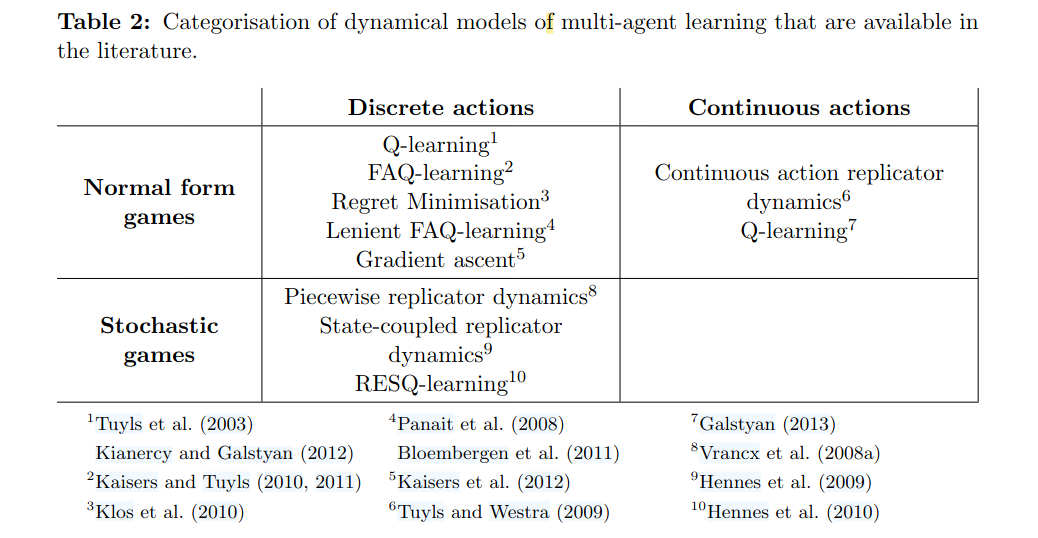
\includegraphics[scale=0.30]{Dynamics setting.png}
    \caption{\citet{bloembergen_evolutionary_2015} Evolutionary
Dynamics of Multi-Agent Learning: A Survey}
  \end{figure}
\end{frame}

\begin{frame}{Evolutionnary game theory}
  \begin{figure}
    \centering
    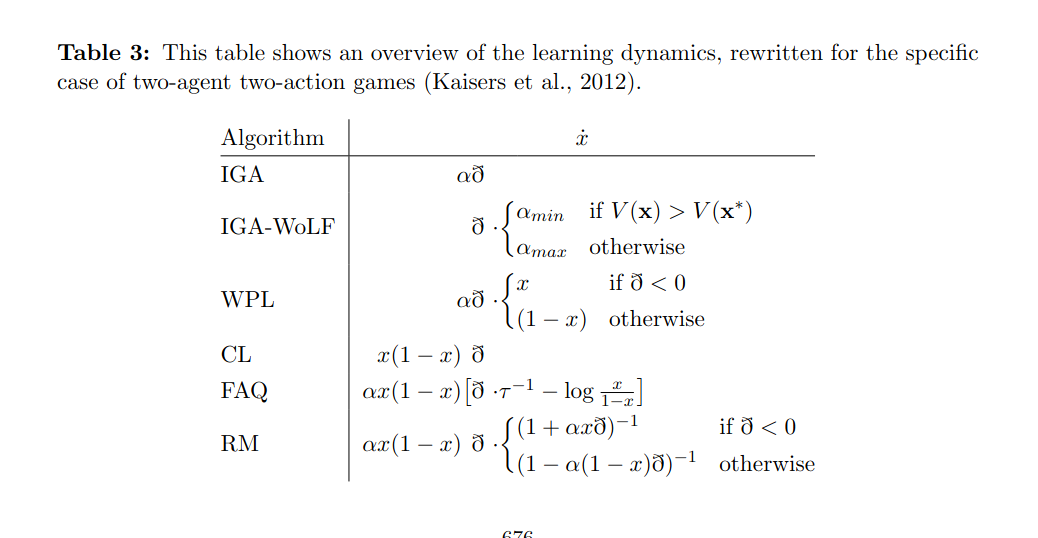
\includegraphics[scale=0.30]{Gradient.png}
    \caption{\citet{bloembergen_evolutionary_2015} Evolutionary
Dynamics of Multi-Agent Learning: A Survey}
  \end{figure}
\end{frame}

\begin{frame}{Evolutionnary game theory}
  \begin{figure}
    \centering
    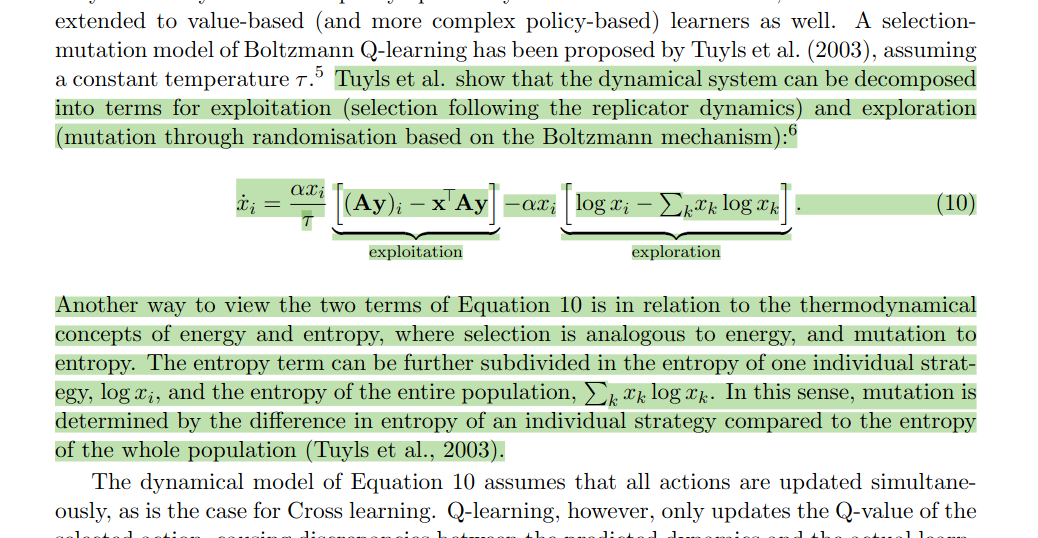
\includegraphics[scale=0.30]{Équation dynamique système.png}
    \caption{\citet{bloembergen_evolutionary_2015} Evolutionary
Dynamics of Multi-Agent Learning: A Survey}
  \end{figure}
\end{frame}

\begin{frame}{Evolutionnary game theory}
  \begin{figure}
    \centering
    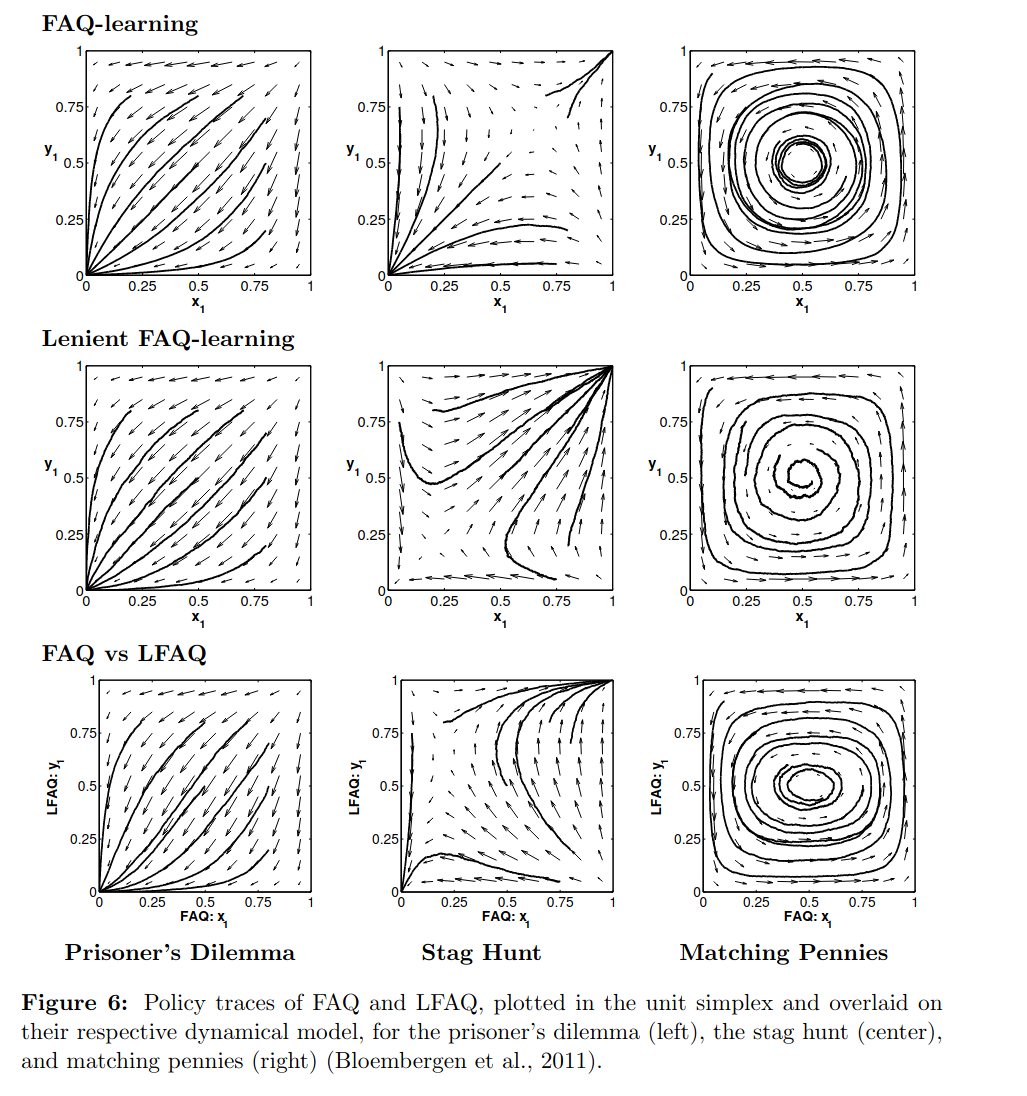
\includegraphics[scale=0.15]{Simplex.png}
    \caption{\citet{bloembergen_evolutionary_2015} Evolutionary
Dynamics of Multi-Agent Learning: A Survey}
  \end{figure}
\end{frame}

\begin{frame}{Non-stationnarité en multi-agent}
  \begin{figure}
    \centering
    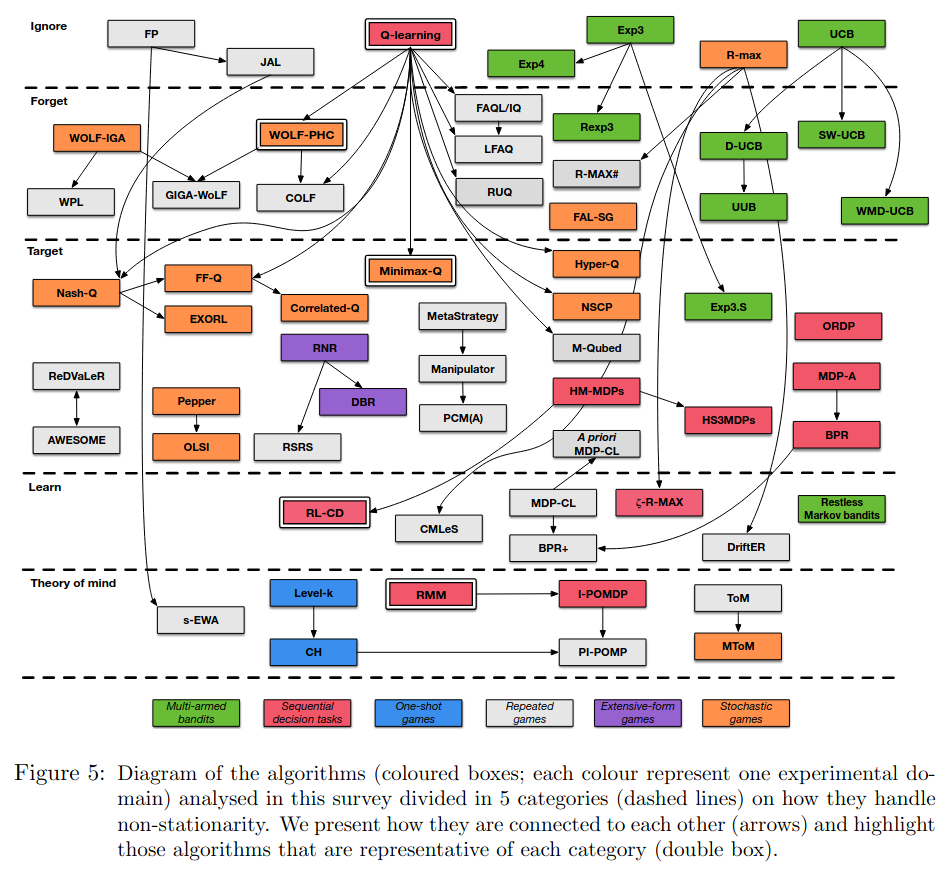
\includegraphics[scale=0.20]{algomultiagent.png}
    \caption{\citet{hernandez-leal_survey_2019} A Survey of Learning in Multiagent Environments:  Dealing with Non-Stationarity}
  \end{figure}
\end{frame}

\begin{frame}{Non-coordination en Markov game}
  \begin{figure}
    \centering
    \includegraphics[scale=0.20]{Définition Markov game.png}
    \caption{\citet{matignon_independent_2012} Independent reinforcement learners in cooperative Markov games: a survey regarding coordination problems}
  \end{figure}
\end{frame}

\begin{frame}{Non-coordination en Markov game}
  \begin{figure}
    \centering
    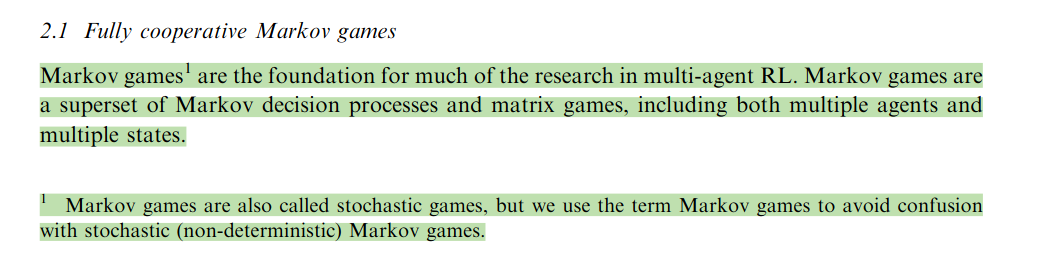
\includegraphics[scale=0.20]{Lien MDP.png}
    \caption{\citet{matignon_independent_2012} Independent reinforcement learners in cooperative Markov games: a survey regarding coordination problems}
  \end{figure}
\end{frame}

\begin{frame}{Non-coordination en Markov game}
  \begin{figure}
    \centering
    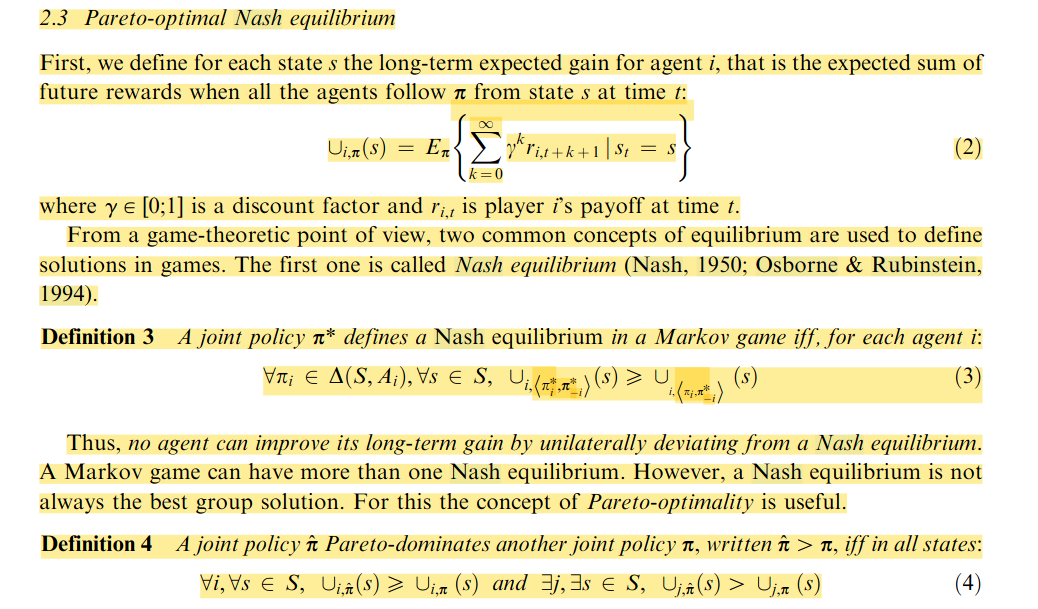
\includegraphics[scale=0.20]{Définition équilibre.png}
    \caption{\citet{matignon_independent_2012} Independent reinforcement learners in cooperative Markov games: a survey regarding coordination problems}
  \end{figure}
\end{frame}

\begin{frame}{Non-coordination en Markov game}
  \begin{figure}
    \centering
    \includegraphics[scale=0.20]{Problème 1.png}
    \caption{\citet{matignon_independent_2012} Independent reinforcement learners in cooperative Markov games: a survey regarding coordination problems}
  \end{figure}
\end{frame}

\begin{frame}{Non-coordination en Markov game}
  \begin{figure}
    \centering
    \includegraphics[scale=0.20]{Problème 2.png}
    \caption{\citet{matignon_independent_2012} Independent reinforcement learners in cooperative Markov games: a survey regarding coordination problems}
  \end{figure}
\end{frame}

\begin{frame}{Non-coordination en Markov game}
  \begin{figure}
    \centering
    \includegraphics[scale=0.20]{Problème 3.png}
    \caption{\citet{matignon_independent_2012} Independent reinforcement learners in cooperative Markov games: a survey regarding coordination problems}
  \end{figure}
\end{frame}

\begin{frame}{Non-coordination en Markov game}
  \begin{figure}
    \centering
    \includegraphics[scale=0.20]{Problème 4.png}
    \caption{\citet{matignon_independent_2012} Independent reinforcement learners in cooperative Markov games: a survey regarding coordination problems}
  \end{figure}
\end{frame}

\begin{frame}{Non-coordination en Markov game}
  \begin{figure}
    \centering
    \includegraphics[scale=0.20]{Problème 5.png}
    \caption{\citet{matignon_independent_2012} Independent reinforcement learners in cooperative Markov games: a survey regarding coordination problems}
  \end{figure}
\end{frame}

\begin{frame}{Non-coordination en Markov game}
  \begin{figure}
    \centering
    \includegraphics[scale=0.20]{Problème 5.png}
    \caption{\citet{matignon_independent_2012} Independent reinforcement learners in cooperative Markov games: a survey regarding coordination problems}
  \end{figure}
\end{frame}

\begin{frame}{Non-coordination en Markov game}
  \begin{figure}
    \centering
    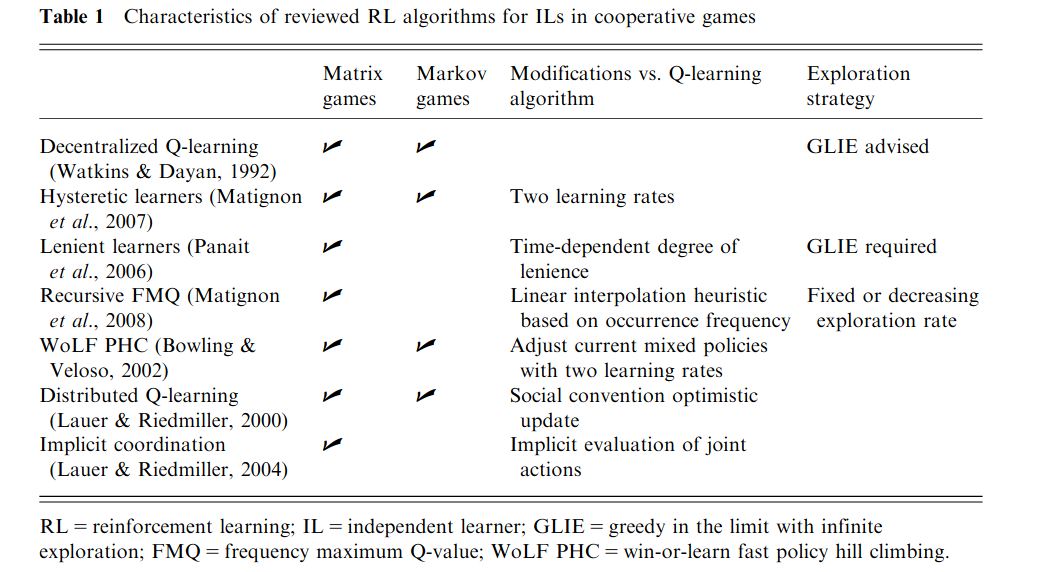
\includegraphics[scale=0.20]{algo modification.png}
    \caption{\citet{matignon_independent_2012} Independent reinforcement learners in cooperative Markov games: a survey regarding coordination problems}
  \end{figure}
\end{frame}

\begin{frame}{Non-coordination en Markov game}
  \begin{figure}
    \centering
    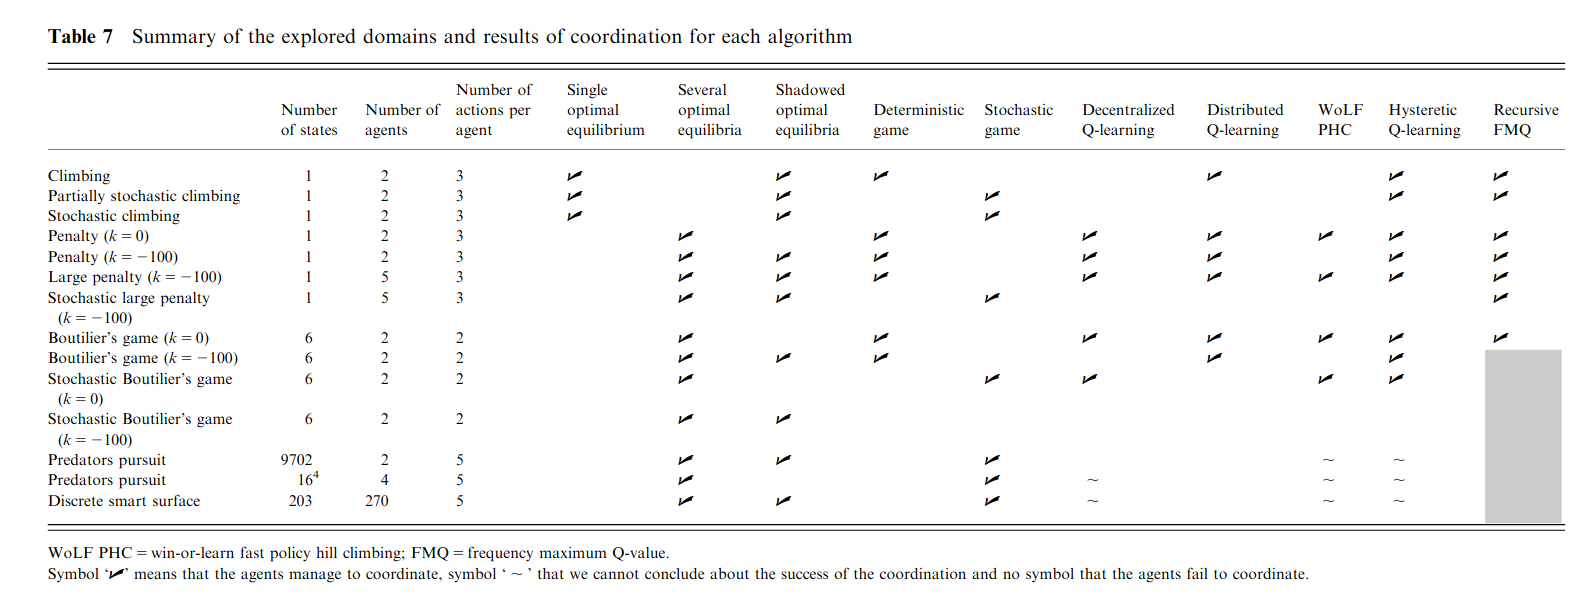
\includegraphics[scale=0.20]{Jeu et performance agent.png}
    \caption{\citet{matignon_independent_2012} Independent reinforcement learners in cooperative Markov games: a survey regarding coordination problems}
  \end{figure}
\end{frame}

\begin{frame}{Non-coordination en Markov game}
  \begin{figure}enn
    \centering
    \includegraphics[scale=0.20]{selon les types de problèmes.png}
    \caption{\citet{matignon_independent_2012} Independent reinforcement learners in cooperative Markov games: a survey regarding coordination problems}
  \end{figure}
\end{frame}

\begin{frame}{Non-coordination en Markov game}
  \begin{figure}
    \centering
    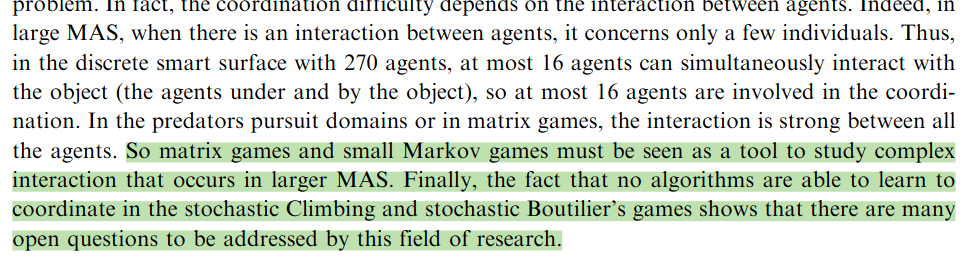
\includegraphics[scale=0.20]{Encouragement.png}
    \caption{\citet{matignon_independent_2012} Independent reinforcement learners in cooperative Markov games: a survey regarding coordination problems}
  \end{figure}
\end{frame}




\section{Organisation articles}


\begin{frame}{Stat}
  \begin{figure}
    \centering
    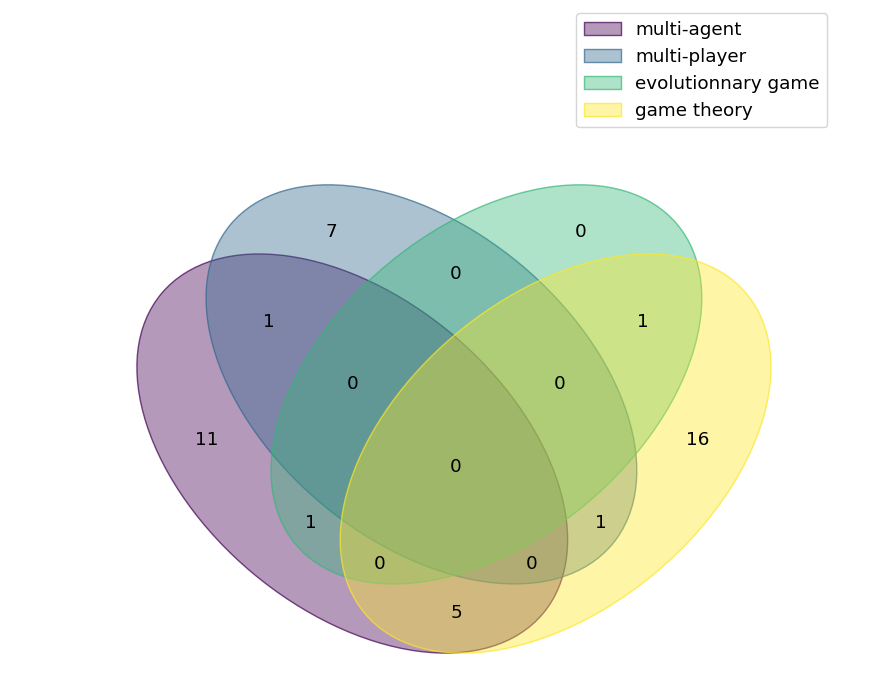
\includegraphics[scale=0.20]{venn.png}
    \caption{}
  \end{figure}
\end{frame}

\begin{frame}{Stat}
  \begin{figure}
    \centering
    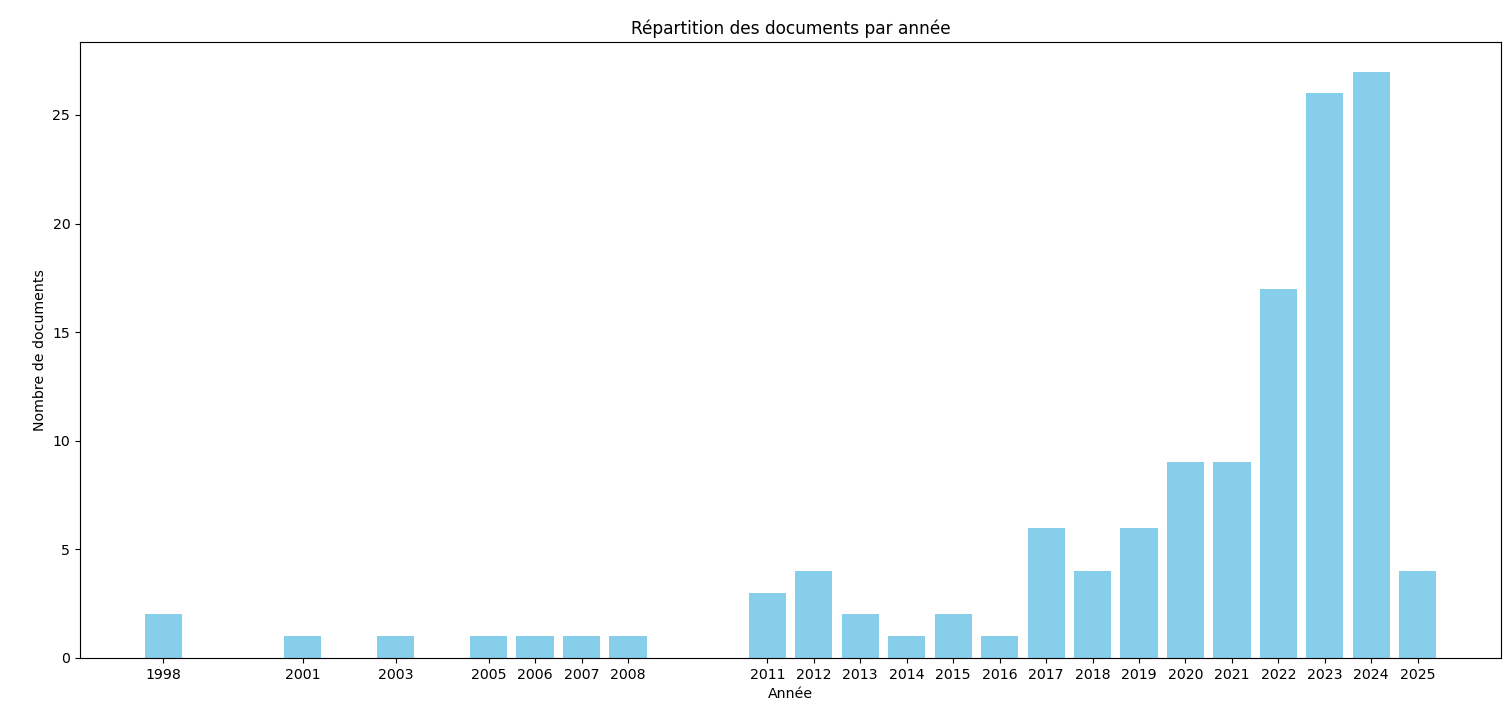
\includegraphics[scale=0.20]{Annee.png}
    \caption{}
  \end{figure}
\end{frame}




















\begin{frame}{Replicator Dynamics}
\begin{itemize}
    \item \citet{mertikopoulos_nested_2024} --- \textit{Nested Replicator Dynamics, Nested Logit Choice, and Similarity-Based Learning}
    \item \citet{fujimoto_learning_2023} --- \textit{Learning in Multi-Memory Games Triggers Complex Dynamics Diverging from Nash Equilibrium}
    \item \citet{tuyls_evolutionary_2005} --- \textit{Evolutionary Game Theory and Multi-Agent Reinforcement Learning}
\end{itemize}
\end{frame}

\begin{frame}{Jeux de Markov}
\begin{itemize}
    \item \citet{matignon_independent_2012} --- \textit{Independent Reinforcement Learners in Cooperative Markov Games: A Survey of Coordination Challenges}
\end{itemize}
\end{frame}

\begin{frame}{Jeux Répétés}
\begin{itemize}
    \item \citet{crandall_learning_2011} --- \textit{Learning to Compete, Coordinate, and Cooperate in Repeated Games Using Reinforcement Learning}
    \item \citet{lin_online_2022} --- \textit{Online Learning in Iterated Prisoner’s Dilemma to Mimic Human Behavior}
    \item \citet{press_iterated_2012} --- \textit{Iterated Prisoner’s Dilemma Contains Strategies that Dominate Any Evolutionary Opponent}
\end{itemize}
\end{frame}

\begin{frame}{Multi-agent Bandit}
\begin{itemize}
    \item \citet{wang_decision_2022} --- \textit{Decision Market Based Learning for Multi-Agent Contextual Bandit Problems}
    \item \citet{xu_regret_2023} --- \textit{Regret Lower Bounds in Multi-Agent Multi-Armed Bandit Problems}
    \item \citet{leshem_fair_2024} --- \textit{Fair Multi-Agent Bandit}
\end{itemize}
\end{frame}

\begin{frame}{Multi-player Bandit}
\begin{itemize}
    \item \citet{boursier_survey_nodate} --- \textit{A Survey on Multi-Player Bandits}
    \item \citet{bistritz_one_2021} --- \textit{One for All and All for One: Distributed Learning of Fair Allocations with Multi-Player Bandits}
    \item \citet{bistritz_my_2020} --- \textit{My Fair Bandit: Distributed Learning of Max-Min Fairness with Multi-Player Bandits}
    \item \citet{bistritz_distributed_2018} --- \textit{Distributed Multi-Player Bandits -- A Game of Thrones Approach}
    \item \citet{bistritz_cooperative_2020} --- \textit{Cooperative Multi-Player Bandit Optimization}
    \item \citet{gursoy_multi-armed_2024} --- \textit{Multi-Armed Bandit Games}
\end{itemize}
\end{frame}


\section{26 mars 2025}
\begin{frame}{26 mars 2025}
26 mars 2025
\end{frame}


\begin{frame}{Listes des algos qui voient ses actions}
  \begin{figure}
    \centering
    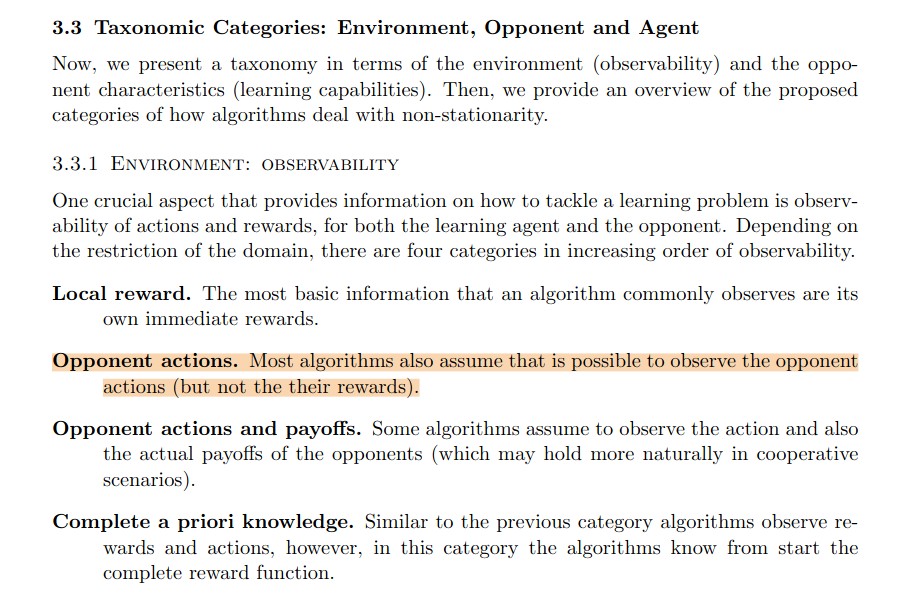
\includegraphics[scale=0.20]{actions_bac.png}
\caption{\citet{hernandez-leal_survey_2019-1} \textit{A Survey of Learning in Multiagent Environments}}
  \end{figure}
\end{frame}

\begin{frame}{Listes des algos qui voient ses actions}
  \begin{figure}
    \centering
    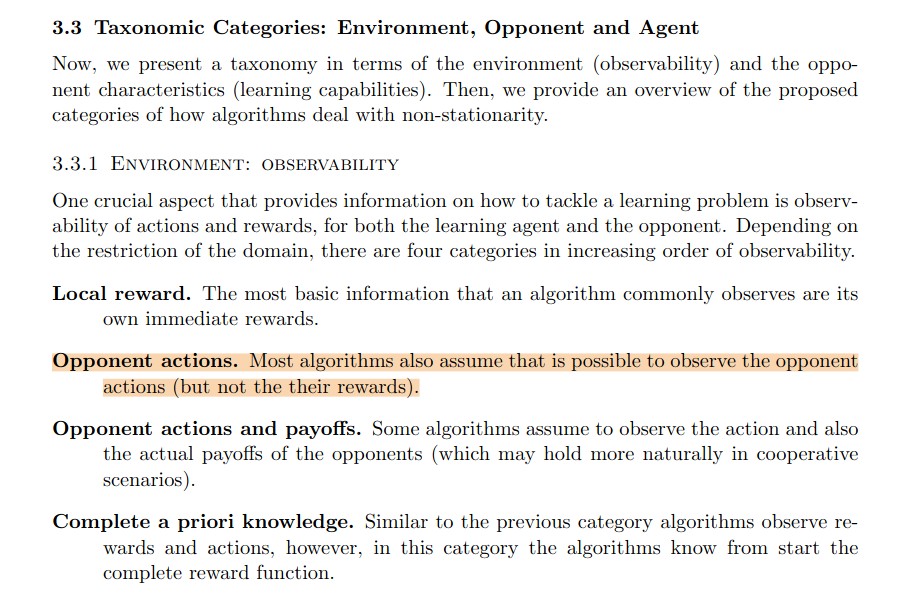
\includegraphics[scale=0.20]{actions_bac.png}
\caption{\citet{hernandez-leal_survey_2019-1} \textit{A Survey of Learning in Multiagent Environments}}
  \end{figure}
\end{frame}

\begin{frame}{Listes des algos qui voient ses actions}
  \begin{figure}
    \centering
    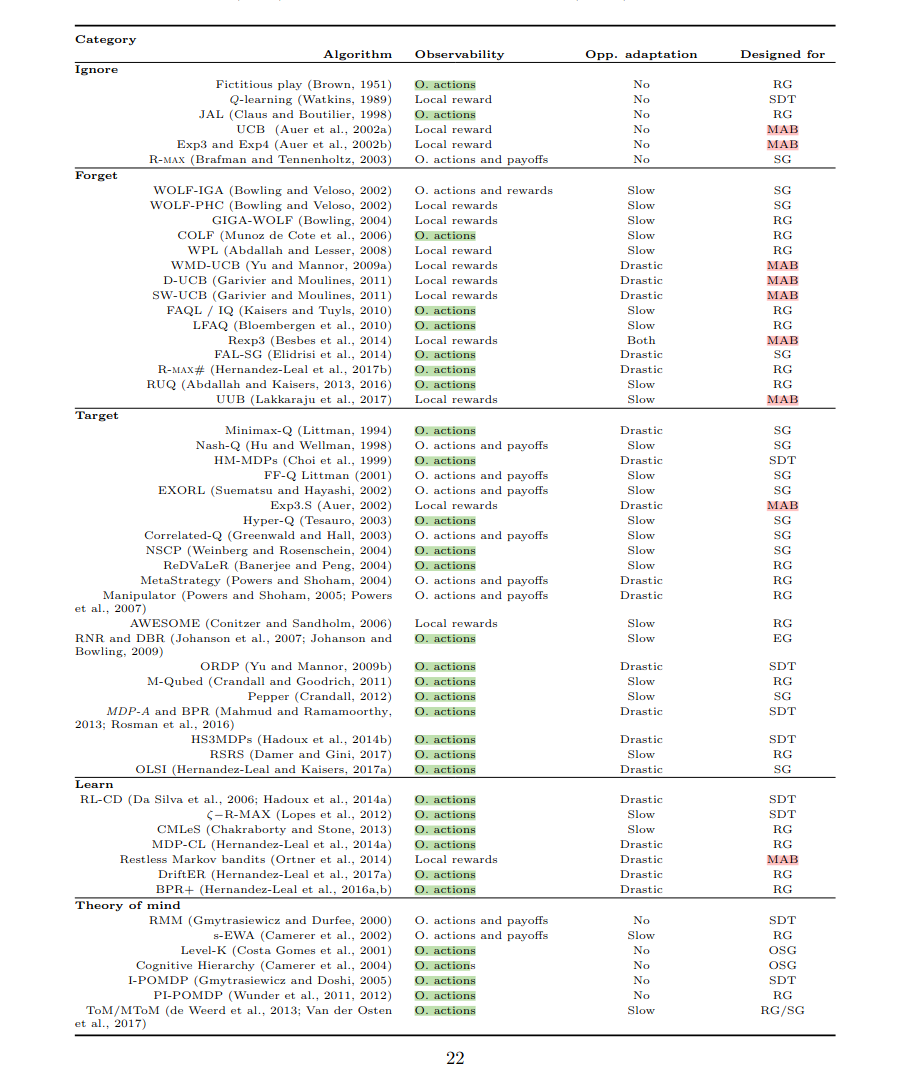
\includegraphics[scale=0.20]{Liste_algo_bac.png}
\caption{\citet{hernandez-leal_survey_2019-1} \textit{A Survey of Learning in Multiagent Environments}}
  \end{figure}
\end{frame}


\begin{frame}{Algorithmes (Forget) qui voient leurs actions}
\begin{itemize}
    \item \textbf{COLF} (Munoz de Cote et al., 2006)
    \item \textbf{FAQL / IQ} (Kaisers and Tuyls, 2010)
    \item \textbf{LFAQ} (Bloembergen et al., 2010)
    \item \textbf{FAL-SG} (Elidrisi et al., 2014)
    \item \textbf{RUQ} (Abdallah and Kaisers, 2013, 2016)
\end{itemize}
\end{frame}


\begin{frame}{Algorithmes (Target) qui voient leurs actions}
\scriptsize
\begin{itemize}
    \item \textbf{Minimax-Q} (Littman, 1994)
    \item \textbf{Nash-Q} (Hu and Wellman, 1998)
    \item \textbf{HM-MDPs} (Choi et al., 1999)
    \item \textbf{PF-Q} (Littman, 2001)
    \item \textbf{EXORL} (Sustermans and Hayashi, 2002)
    \item \textbf{Correlated-Q} (Greenwald and Hall, 2003)
    \item \textbf{NSCP} (Weinberg and Rosenschein, 2004)
    \item \textbf{RNeDLeR} (Banerjee and Peng, 2004)
    \item \textbf{MetaStrategy} (Powers and Shoham, 2004)
    \item \textbf{Manipulator} (Powers and Shoham, 2005; Powers et al., 2007)
    \item \textbf{AWESOME} (Conitzer and Sandholm, 2006)
    \item \textbf{RNR and DBR} (Johanson et al., 2007; Johanson and Bowling, 2009)
    \item \textbf{ORDP} (Yu and Mannor, 2009)
    \item \textbf{M-Qubed} (Crandall and Goodrich, 2011)
    \item \textbf{Pepper} (Crandall, 2012)
    \item \textbf{MDP-A and BPR} (Mahmoud and Ramaonarothy, 2013; Rosman et al., 2016)
    \item \textbf{H3MSDPs} (Hadoux et al., 2014b)
    \item \textbf{MSRS} (Daeme and Gini, 2017)
    \item \textbf{OLSI} (Hernandez-Leal and Kaisers, 2017c)
\end{itemize}
\end{frame}


\begin{frame}{Algorithmes (Learn) qui voient leurs actions}
\begin{itemize}
    \item \textbf{RC-MAX\#} (Hernandez-Leal et al., 2014c)
    \item \textbf{DriftER} (Hernandez-Leal et al., 2017a)
    \item \textbf{BPR+} (Hernandez-Leal et al., 2016a,b)
\end{itemize}
\end{frame}

\begin{frame}{Algorithmes (Theory of Mind) qui voient leurs actions}
\begin{itemize}
    \item \textbf{I-POMDP} (Gmytrasiewicz and Doshi, 2005)
    \item \textbf{PI-POMDP} (Wunder et al., 2011)
    \item \textbf{ToM/MTOM} (de Weerd et al., 2013; Van der Osten et al., 2017)
\end{itemize}
\end{frame}

\begin{frame}{Algorithmes (Ignore) avec Local reward}
\begin{itemize}
    \item \textbf{Q-learning} (Watkins, 1989)
    \item \textbf{JAL} (Claus and Boutilier, 1998)
    \item \textbf{UCB} (Auer et al., 2002a)
    \item \textbf{Exp3 and Exp4} (Auer et al., 2002b)
\end{itemize}
\end{frame}

\begin{frame}{Algorithmes (Forget) avec Local reward}
\begin{itemize}
    \item \textbf{WPL} (Abdallah and Lesser, 2008)
    \item \textbf{D-UCB} (Garivier and Moulines, 2011)
    \item \textbf{SW-UCB} (Garivier and Moulines, 2011)
    \item \textbf{UUB} (Lakkaraju et al., 2017)
\end{itemize}
\end{frame}

\begin{frame}{Algorithmes (Learn) avec Local reward}
\begin{itemize}
    \item \textbf{Restless Markov Bandits} (Otter et al., 2014)
\end{itemize}
\end{frame}


\begin{frame}{références}
\bibliographystyle{plainnat}
\bibliography{references}
\end{frame}
% %------------------------------------------------
% \begin{frame}{Blocks of Highlighted Text}
%     In this slide, some important text will be \alert{highlighted} because it's important. Please, don't abuse it.

%     \begin{block}{Block}
%         Sample text
%     \end{block}

%     \begin{alertblock}{Alertblock}
%         Sample text in red box
%     \end{alertblock}

%     \begin{examples}
%         Sample text in green box. The title of the block is ``Examples".
%     \end{examples}
% \end{frame}

% %------------------------------------------------

% \begin{frame}{Multiple Columns}
%     \begin{columns}[c] % The "c" option specifies centered vertical alignment while the "t" option is used for top vertical alignment

%         \column{.45\textwidth} % Left column and width
%         \textbf{Heading}
%         \begin{enumerate}
%             \item Statement
%             \item Explanation
%             \item Example
%         \end{enumerate}

%         \column{.45\textwidth} % Right column and width
%         Lorem ipsum dolor sit amet, consectetur adipiscing elit. Integer lectus nisl, ultricies in feugiat rutrum, porttitor sit amet augue. Aliquam ut tortor mauris. Sed volutpat ante purus, quis accumsan dolor.

%     \end{columns}
% \end{frame}

% %------------------------------------------------
% \section{Second Section}
% %------------------------------------------------

% \begin{frame}{Table}
%     \begin{table}
%         \begin{tabular}{l l l}
%             \toprule
%             \textbf{Treatments} & \textbf{Response 1} & \textbf{Response 2} \\
%             \midrule
%             Treatment 1         & 0.0003262           & 0.562               \\
%             Treatment 2         & 0.0015681           & 0.910               \\
%             Treatment 3         & 0.0009271           & 0.296               \\
%             \bottomrule
%         \end{tabular}
%         \caption{Table caption}
%     \end{table}
% \end{frame}

% %------------------------------------------------

% \begin{frame}{Theorem}
%     \begin{theorem}[Mass--energy equivalence]
%         $E = mc^2$
%     \end{theorem}
% \end{frame}

% %------------------------------------------------

% \begin{frame}{Figure}
%     Uncomment the code on this slide to include your own image from the same directory as the template .TeX file.
%     %\begin{figure}
%     %\includegraphics[width=0.8\linewidth]{test}
%     %\end{figure}
% \end{frame}

% %------------------------------------------------

% \begin{frame}[fragile] % Need to use the fragile option when verbatim is used in the slide
%     \frametitle{Citation}
%     An example of the \verb|\cite| command to cite within the presentation:\\

%     This statement requires citation \cite{p1}.
% \end{frame}

% %------------------------------------------------

% \begin{frame}{References}
%     \footnotesize
%     \bibliography{reference.bib}
%     \bibliographystyle{apalike}
% \end{frame}

% %------------------------------------------------

% \begin{frame}
%     \Huge{\centerline{\textbf{The End}}}
% \end{frame}

% %----------------------------------------------------------------------------------------

\end{document}
